% =========================================================
% AfricaBP — bioAI Workshop · Atelier pratique 2026
% Pitch de 5 minutes pour présenter le projet aux étudiants
%
% Compilation : pdflatex main.tex (2x), ou directement sur Overleaf.
% Aucune image externe : toutes les figures sont en TikZ.
% =========================================================
\documentclass[11pt,aspectratio=169]{beamer}

\usetheme{metropolis}
\makeatletter
\setbeamertemplate{frametitle}{%
  \nointerlineskip
  \begin{beamercolorbox}[wd=\paperwidth,ht=4ex,dp=2.5ex,
                         leftskip=0.7cm,rightskip=0.3cm]{frametitle}
    \usebeamerfont{frametitle}\insertframetitle
  \end{beamercolorbox}
}
\makeatother

\usepackage[french]{babel}
\usepackage[utf8]{inputenc}
\usepackage[T1]{fontenc}
\usepackage{tikz}
\usetikzlibrary{arrows.meta,positioning,fit,backgrounds,calc}
\usetikzlibrary{overlay-beamer-styles}   % clé alt=<n>{...}{...} pour les overlays
\usepackage[most]{tcolorbox}
\usepackage{xcolor}
\usepackage[normalem]{ulem}   % \sout : texte barré

% ---- palette (reprise du template académique) -----------
\definecolor{aliveblue}{RGB}{20,60,110}
\definecolor{alivegold}{RGB}{198,146,20}
\definecolor{alivegray}{RGB}{90,90,90}
\definecolor{alivegreen}{RGB}{30,110,60}

\setbeamercolor{palette primary}{bg=aliveblue,fg=white}
\setbeamercolor{frametitle}{bg=white,fg=aliveblue}
\setbeamercolor{progress bar}{fg=alivegold,bg=aliveblue!20}
\setbeamercolor{alerted text}{fg=alivegold}
\setbeamertemplate{itemize item}{\color{alivegold}\textbullet}
\setbeamertemplate{navigation symbols}{}

\setbeamertemplate{footline}{%
  \leavevmode\hbox{%
    \begin{beamercolorbox}[wd=.90\paperwidth,ht=3.2ex,dp=3ex,leftskip=10pt]{normal text}
      \scriptsize\color{alivegray}\insertsectionhead
    \end{beamercolorbox}%
    \begin{beamercolorbox}[wd=.10\paperwidth,ht=3.2ex,dp=3ex,center]{normal text}
      \tikz[baseline=(n.base)]{\node[fill=alivegold,rounded corners=2pt,
        minimum width=9mm,minimum height=9mm,inner xsep=1.5pt,inner ysep=5pt,
        text=white,font=\bfseries\scriptsize] (n)
        {\insertframenumber{\tiny/\inserttotalframenumber}};}
    \end{beamercolorbox}}%
}

% ---- briques réutilisables ------------------------------
\tikzset{
  bx/.style   = {draw=aliveblue,rounded corners,thick,fill=white,
                 minimum width=#1,minimum height=1.05cm,align=center,font=\scriptsize},
  bx/.default = 2.3cm,
  fbx/.style  = {draw=aliveblue,rounded corners,thick,fill=aliveblue,text=white,
                 minimum width=#1,minimum height=1.05cm,align=center,font=\scriptsize},
  fbx/.default= 2.3cm,
  gbx/.style  = {draw=alivegold,rounded corners,thick,dashed,fill=white,
                 minimum width=#1,minimum height=1.05cm,align=center,font=\scriptsize},
  gbx/.default= 2.3cm,
  arr/.style  = {-{Latex[length=2.2mm]},thick,alivegold},
}
\newtcolorbox{keybox}[1]{colback=alivegold!7,colframe=alivegold,arc=2mm,
  boxrule=0.8pt,left=3mm,right=3mm,top=2mm,bottom=2mm,title=#1,
  fonttitle=\bfseries\small,coltitle=alivegold,colbacktitle=alivegold!7}
\newtcolorbox{navybox}[1]{colback=aliveblue!6,colframe=aliveblue,arc=2mm,
  boxrule=0.8pt,left=3mm,right=3mm,top=2mm,bottom=2mm,title=#1,
  fonttitle=\bfseries\small,coltitle=aliveblue,colbacktitle=aliveblue!6}

% ---- métadonnées ----------------------------------------
\usepackage{graphicx}
\title{Classificateur de fonction de protéines}
\subtitle{IA et Biologie : de la compréhension de l'ADN à la distillation de modèles}
\date{}

\begin{document}

% =========================================================
{\setbeamercolor{background canvas}{bg=aliveblue}
 \setbeamertemplate{footline}{}
\begin{frame}[plain]
  \begin{tikzpicture}[remember picture,overlay]
    % --- hélice d'ADN à droite, débordant du bord de la page
    % dna-light.png = silhouette blanche dérivée de dna.png (le PNG d'origine est
    % bleu foncé, donc invisible sur ce fond navy). Régénérable avec :
    %   magick dna.png -alpha extract -write mask.png +delete \
    %     \( -size 1200x1200 xc:white \) mask.png -alpha off \
    %     -compose copy_opacity -composite dna-light.png
    \node[anchor=east,opacity=0.42,inner sep=0pt]
      at ([xshift=1.7cm]current page.east)
      {
\includegraphics[height=1.06\paperheight]{illustrations/dna-light.png}};

    % --- logo de l'école, sur une carte noire (le PNG est transparent)
    \node[fill=black,rounded corners=3pt,inner sep=6pt,anchor=north west]
      at ([shift={(0.95,-0.75)}]current page.north west)
      {
\includegraphics[width=2.8cm]{illustrations/background-logo.png}};

    % --- bloc titre
    \node[anchor=west,text width=10.4cm,align=left]
      at ([shift={(1.05,-0.95)}]current page.west) {
      {\color{white}\fontsize{30}{30.5}\selectfont\bfseries
       Classificateur de fonction de protéines\par}
      \vspace{0.22cm}
      {\color{white!78}\fontsize{14}{15}\selectfont
       IA et Biologie : de la compréhension de l'ADN\\
       à la distillation de modèles\par}
      \vspace{0.85cm}
      {\color{alivegold}\footnotesize\bfseries
       ATELIER bioIA AfricaBP \quad·\quad 28 -- 29 OCTOBRE 2026\par}
    };
  \end{tikzpicture}
\end{frame}}
\addtocounter{framenumber}{-1}

% =========================================================
\section{Le problème}

% <<<<<<<< LA BIOLOGIE EN UNE SLIDE >>>>>>>>
% NOTE : copiez dogma.png dans illustrations/ (il vient de l'ancien template).
\begin{frame}{De l'ADN à la protéine : le dogme central}
  \begin{columns}[T]
    \begin{column}{0.58\textwidth}
      \textbf{Trois étapes, toujours les mêmes}

      \begin{itemize}\small
        \item<1-> \textbf{L'ADN} stocke l'information, écrite avec quatre lettres :
              A, T, G, C
        \item<2-> \textbf{La transcription} en recopie un morceau en ARN
        \item<3-> \textbf{La traduction} lit cet ARN \emph{trois lettres à la fois}, chaque triplet (codon) désigne un acide aminé, et la chaîne d'acides aminés forme une \textbf{protéine}
      \end{itemize}

      \only<4->{
      \begin{tcolorbox}[colback=alivegold!8,colframe=alivegold,arc=2mm,
                        boxrule=0.8pt,left=3mm,right=3mm,top=2mm,bottom=2mm]
      \textbf{\color{alivegold}Ce qu'il faut retenir}

      Seules certaines portions de l'ADN suivent ce chemin jusqu'à la protéine :
      ces portions particulières, ce sont les \textbf{gènes}.
      \end{tcolorbox}
      }
    \end{column}
    \begin{column}{0.42\textwidth}
      \centering
      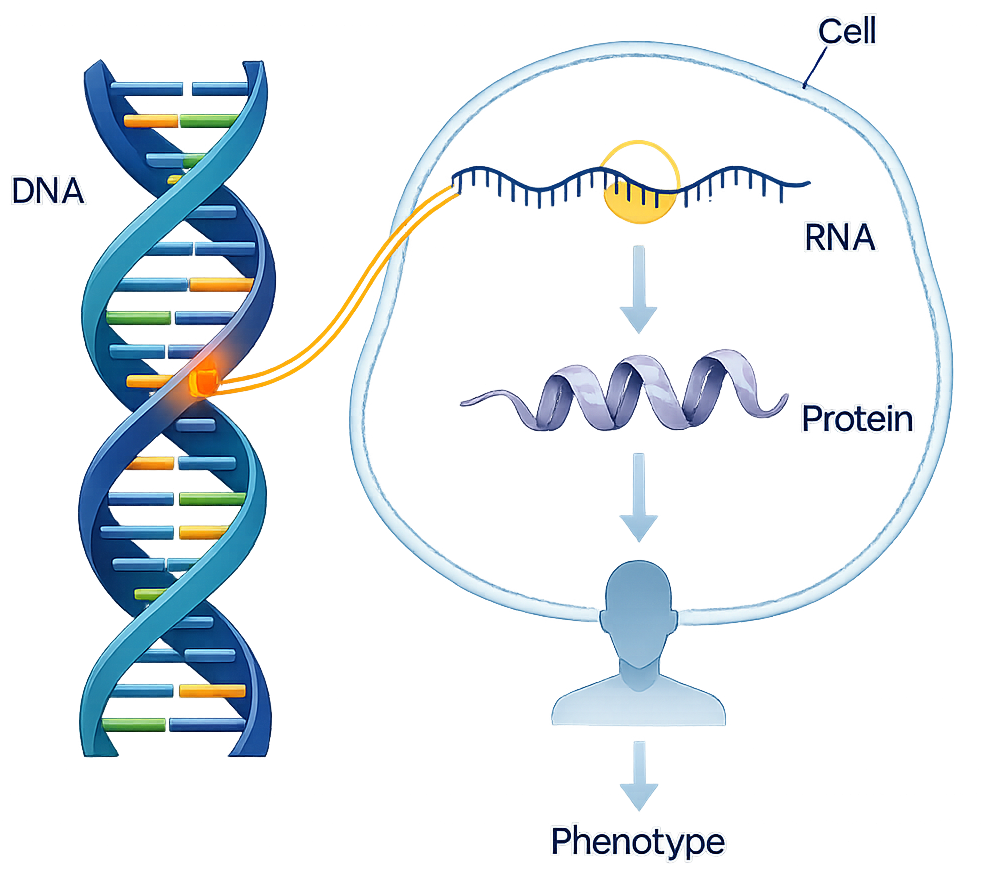
\includegraphics[width=\linewidth]{illustrations/dogma.png}
    \end{column}
  \end{columns}
\end{frame}

\begin{frame}{Où sont les gènes ?}
  \begin{columns}[T,onlytextwidth]
    \begin{column}{0.54\textwidth}
      \begin{itemize}\small
        \item {\color{alivegray}\sout{Humain}} \quad
              {\color{alivegray}\sout{Plante}} \quad
              \textbf{Bactérie} \\[2pt]
              {\footnotesize nous travaillons avec des \textbf{bactéries} :
               des génomes petits et bien annotés}
        \item Leur génome, c'est \textbf{des millions de lettres} à la suite :
              [3pt]
              {\ttfamily\footnotesize
               \ldots ATGCTAGCTAGGCCGGCATG \ldots}
        \item \textbf{Rien ne les sépare visuellement.}
              Pas de titres, pas d'espaces.
      \end{itemize}
      \medskip

      \begin{keybox}{La question de l'atelier}
        \small Notre tâche : \textbf{prédire où se trouvent les gènes}.
        On vous donne 200 lettres d'ADN --- est-ce un morceau de gène,
        oui ou non ?
      \end{keybox}
    \end{column}
    \begin{column}{0.44\textwidth}
      \centering
      \begin{tikzpicture}[scale=0.92,every node/.style={font=\tiny}]
        \draw[fill=aliveblue!6,draw=aliveblue!25] (0,3.1) rectangle (6.2,3.7);
        \draw[fill=aliveblue,draw=aliveblue]      (0.7,3.1) rectangle (2.4,3.7);
        \draw[fill=alivegreen,draw=alivegreen]    (3.5,3.1) rectangle (4.9,3.7);
        \node[white] at (1.55,3.4) {\bfseries GÈNE};
        \node[white] at (4.2,3.4)  {\bfseries GÈNE};
        \node[alivegray] at (2.95,3.4) {non-codant};

        \draw[alivegold,thick] (3.5,3.05) -- (3.5,2.6) -- (4.9,2.6) -- (4.9,3.05);
        \draw[arr] (4.2,2.6) -- (4.2,2.15);

        \draw[fill=white,draw=aliveblue!25,rounded corners]
              (0,1.35) rectangle (6.2,2.05);
        \node[font=\ttfamily\scriptsize] at (3.1,1.7) {ATGCTAGCTAGGCATCGA\ldots};

        \draw[fill=alivegreen!12,draw=alivegreen,rounded corners]
              (0,0.3) rectangle (2.95,1.0);
        \node[alivegreen] at (1.47,0.65) {\bfseries GÈNE ?};
        \draw[fill=black!4,draw=alivegray,rounded corners]
              (3.25,0.3) rectangle (6.2,1.0);
        \node[alivegray] at (4.72,0.65) {\bfseries PAS UN GÈNE ?};
      \end{tikzpicture}
    \end{column}
  \end{columns}
\end{frame}

% =========================================================
\begin{frame}{Ce n'est pas un exercice d'école}
  \begin{columns}[T,onlytextwidth]
    \begin{column}{0.55\textwidth}
      \small
      Chaque fois qu'un nouvel organisme est séquencé --- une bactérie résistante
      aux antibiotiques, un virus, un microbe du sol --- \textbf{quelqu'un doit
      trouver ses gènes}. C'est la première étape de toute la biologie moderne.
      \bigskip

      {\color{alivegray}\normalsize Et personne ne le fait à la main.}
    \end{column}
    \begin{column}{0.42\textwidth}
      \begin{navybox}{Un problème de « trouver l'aiguille »}
        \small Des millions de fenêtres possibles, deux réponses possibles.
        C'est exactement le type de tâche où l'IA est bonne\ldots{} si on lui
        donne la bonne représentation des données.
      \end{navybox}
      \vspace{0.4cm}
      \centering\small
      \begin{tabular}{ccc}
        {\Large\bfseries\color{aliveblue}4} &
        {\Large\bfseries\color{aliveblue}$\sim$4\,M} &
        {\Large\bfseries\color{aliveblue}2}\\[2pt]
        {\tiny\color{alivegray}LETTRES} &
        {\tiny\color{alivegray}PAR GÉNOME} &
        {\tiny\color{alivegray}RÉPONSES}
      \end{tabular}
    \end{column}
  \end{columns}
\end{frame}

% =========================================================
\section{L'idée forte}

% <<<<<<<< UNE NOUVELLE CLASSE DE MODÈLES >>>>>>>>
% NOTE : copiez llm-short.png dans illustrations/ (il vient de l'ancien template).
\begin{frame}{L'opportunité : la biologie a ses propres modèles de langage}
  \vspace{-1cm}
  \hspace{-0.4cm}
  % \textbf{Modéliser une séquence est un excellent prétexte pour apprendre à représenter le vivant.}
  \vspace{6pt}

  \begin{figure}
    \centering
    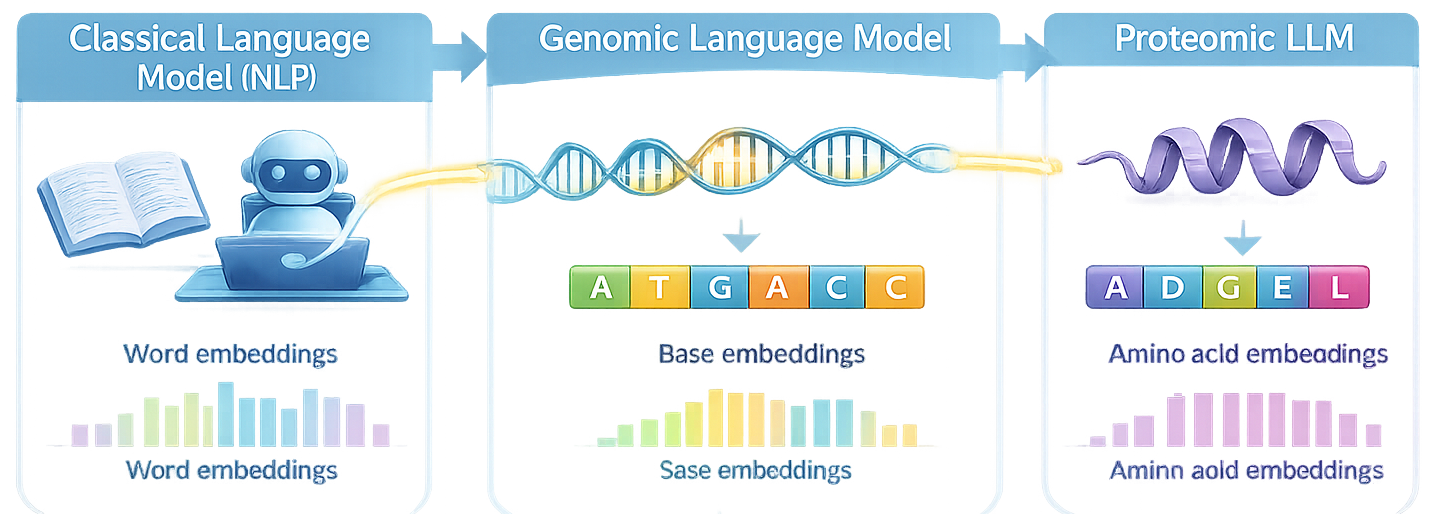
\includegraphics[width=0.85\linewidth]{illustrations/llm-short.png}
  \end{figure}

  \begin{columns}[T,onlytextwidth]
    \begin{column}{0.5\textwidth}
      \centering\small
      \textbf{\textcolor{aliveblue}{Langage naturel}}\\
      Prédire le mot suivant\\
      \emph{GPT : apprend la grammaire, la syntaxe et le sens}
    \end{column}
    \begin{column}{0.5\textwidth}
      \centering\small
      \textbf{\textcolor{aliveblue}{Séquences biologiques}}\\
      Prédire le nucléotide suivant\\
      \emph{DNABERT, Evo2\ldots : apprennent la structure et la fonction
      biologiques}
    \end{column}
  \end{columns}
\end{frame}

\begin{frame}{Evo2 : une représentation riche\ldots{} mais un modèle énorme}
  \begin{columns}[T,onlytextwidth]
    \begin{column}{0.46\textwidth}
      \small
      % \textbf{L'idée} 
      \textbf{L'idée}: on demande à \textbf{Evo2} une \alert{représentation riche} des ADN \& on branche ensuite un petit classifieur dessus
      % \begin{itemize}\small
      %     \item 
      %  \end{itemize}
        
      % : plutôt que de décrire la séquence nous-mêmes, on demande
      % à \textbf{Evo2} une \alert{représentation riche} de chaque fenêtre, et on
      % branche un petit classifieur dessus. Sans surprise, il fait bien mieux que
      % nos baseline.
      \medskip

      \textbf{Le problème} : 7 milliards de paramètres. Impossible à faire tourner
      sur un laptop ou un séquenceur de terrain.
      \medskip

      \begin{keybox}{La solution : la distillation}
        \small Le gros modèle « professeur » entraîne un modèle « élève » minuscule, en lui transmettant non pas la bonne réponse, mais
        \alert{son degré d'hésitation}.
      \end{keybox}
    \end{column}
    \begin{column}{0.52\textwidth}
      \centering
      \begin{tikzpicture}[scale=0.86,every node/.style={font=\tiny}]
        % --- Evo2 -> représentation -> classifieur
        \node[bx=2.2cm] (in) at (1.2,4.5) {200 lettres d'ADN};
        \node[fbx=2.2cm] (ev) at (1.2,3.1) {\bfseries Evo2\\[1pt]
              {\color{alivegold}7 000 000 000}};
        \draw[arr] (in) -- (ev);

        \draw[draw=aliveblue!25,fill=aliveblue!3,rounded corners]
              (3.0,2.3) rectangle (6.6,5.1);
        \node[alivegray] at (4.8,4.9) {représentation apprise};
        \foreach \p in {(3.6,4.4),(3.95,4.6),(3.5,4.05),(3.9,4.15),(4.25,4.5)}
          \fill[alivegreen] \p circle (2.2pt);
        \foreach \p in {(5.6,3.0),(5.95,3.25),(5.35,2.75),(5.8,2.7),(6.15,3.0)}
          \fill[alivegray!70] \p circle (2.2pt);
        \draw[alivegold,thick,dashed] (3.2,2.7) -- (6.4,4.6);
        \node[alivegreen] at (3.45,4.75) {\bfseries gènes};
        \node[alivegray]  at (5.9,2.45)  {\bfseries non-gènes};
        \draw[arr] (ev.east) -- (2.95,3.1);

        % --- professeur -> élève
        \node[fbx=2.6cm] (t) at (1.6,1.35)
             {\bfseries PROFESSEUR\\[1pt]Evo2 + classifieur\\[1pt]
              {\color{alivegold}\bfseries 7 000 000 000}};
        \node[bx=2.6cm] (s) at (5.4,1.35)
             {\bfseries ÉLÈVE\\[1pt]k-mers + petit MLP\\[1pt]
              {\color{alivegold}\bfseries $\sim$70 000}};
        \draw[arr] (t) -- node[above,alivegold,font=\tiny\bfseries] {distillation} (s);
      \end{tikzpicture}
    \end{column}
  \end{columns}
\end{frame}

% =========================================================
\section{Ce que nous construirons}
\begin{frame}{Trois jours, cinq labs + un bonus : un pipeline complet}
  \centering
  \begin{tikzpicture}[node distance=0.28cm,every node/.style={font=\tiny}]
    \node[bx=1.95cm,alt=<1>{fill=alivegold!15,draw=alivegold}{}] (d1)
      {{\color{alivegold}\bfseries LAB 1}\\[2pt]Données\\+ baselines};
    \node[bx=1.95cm,right=of d1,alt=<2>{fill=alivegold!15,draw=alivegold}{}] (d2)
      {{\color{alivegold}\bfseries LAB 2}\\[2pt]Evo2 :\\le professeur};
    \node[bx=1.95cm,right=of d2,alt=<3>{fill=alivegold!15,draw=alivegold}{}] (d3)
      {{\color{alivegold}\bfseries LAB 3}\\[2pt]Distillation\\prof $\rightarrow$ élève};
    \node[bx=1.95cm,right=of d3,alt=<4>{fill=alivegold!15,draw=alivegold}{}] (d4)
      {{\color{alivegold}\bfseries LAB 4}\\[2pt]Le verdict :\\taille vs précision};
    \node[bx=1.95cm,right=of d4,alt=<5>{fill=alivegold!15,draw=alivegold}{}] (d5)
      {{\color{alivegold}\bfseries LAB 5}\\[2pt]Qu'a compris\\le modèle, seul ?};
    \node[gbx=1.95cm,right=of d5,alt=<6>{fill=alivegold!15}{}] (d6)
      {{\color{alivegold}\bfseries LAB BONUS}\\[2pt]Et les protéines ?\\mini-démo ESM2};
    \draw[arr] (d1) -- (d2); \draw[arr] (d2) -- (d3);
    \draw[arr] (d3) -- (d4); \draw[arr] (d4) -- (d5);
    \draw[arr,dashed] (d5) -- (d6);
  \end{tikzpicture}

  \vspace{0.55cm}

  % --- puces orange : elles apparaissent sous le lab dont on parle
  \begin{minipage}[t][3.9cm][t]{0.96\textwidth}
    \small
    \only<1>{%
      \centering
      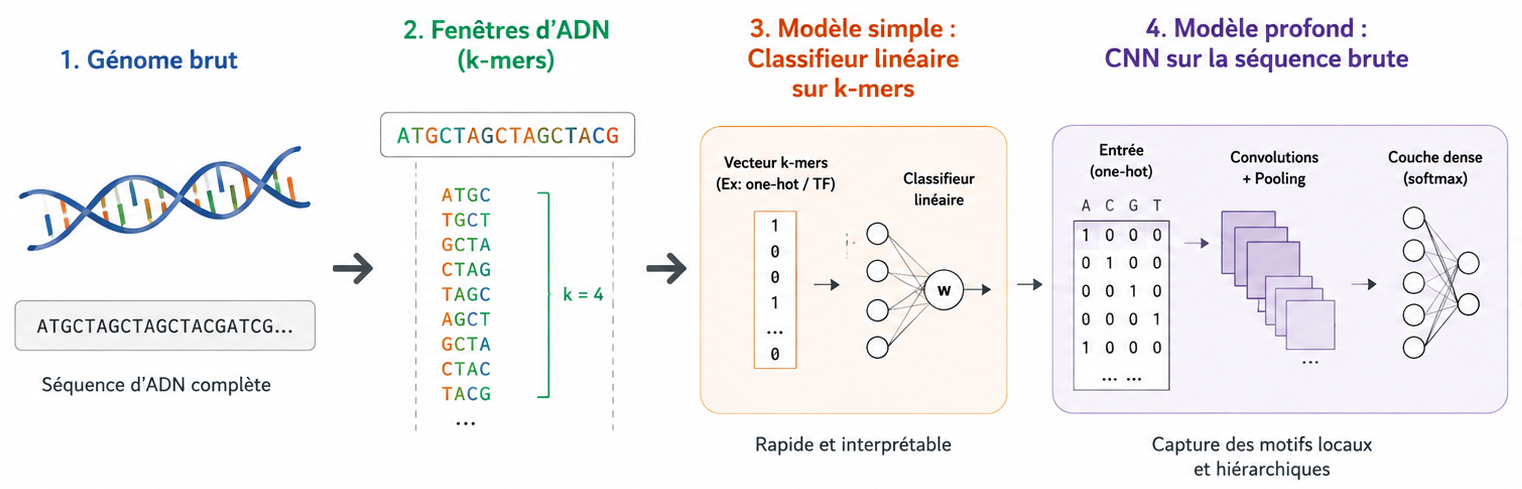
\includegraphics[height=4.2cm,keepaspectratio]{illustrations/lab1.png}}
    \only<2>{%
      \centering
      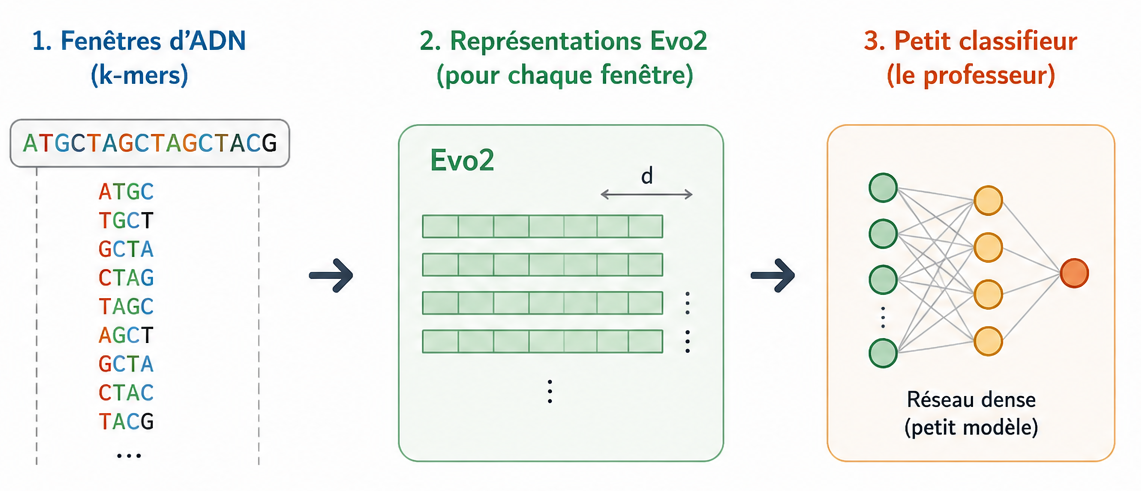
\includegraphics[height=4.2cm,keepaspectratio]{illustrations/lab2.png}\\[4pt]
      % 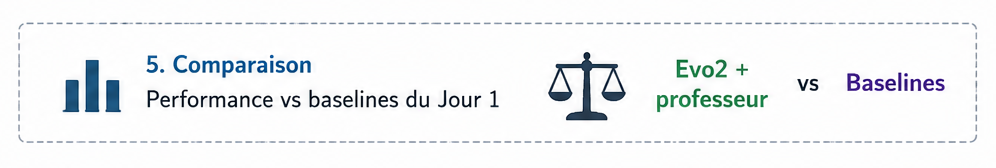
\includegraphics[width=8.5cm,keepaspectratio]{illustrations/lab2-bottom.png}
      }
    \only<3>{%
      \centering
      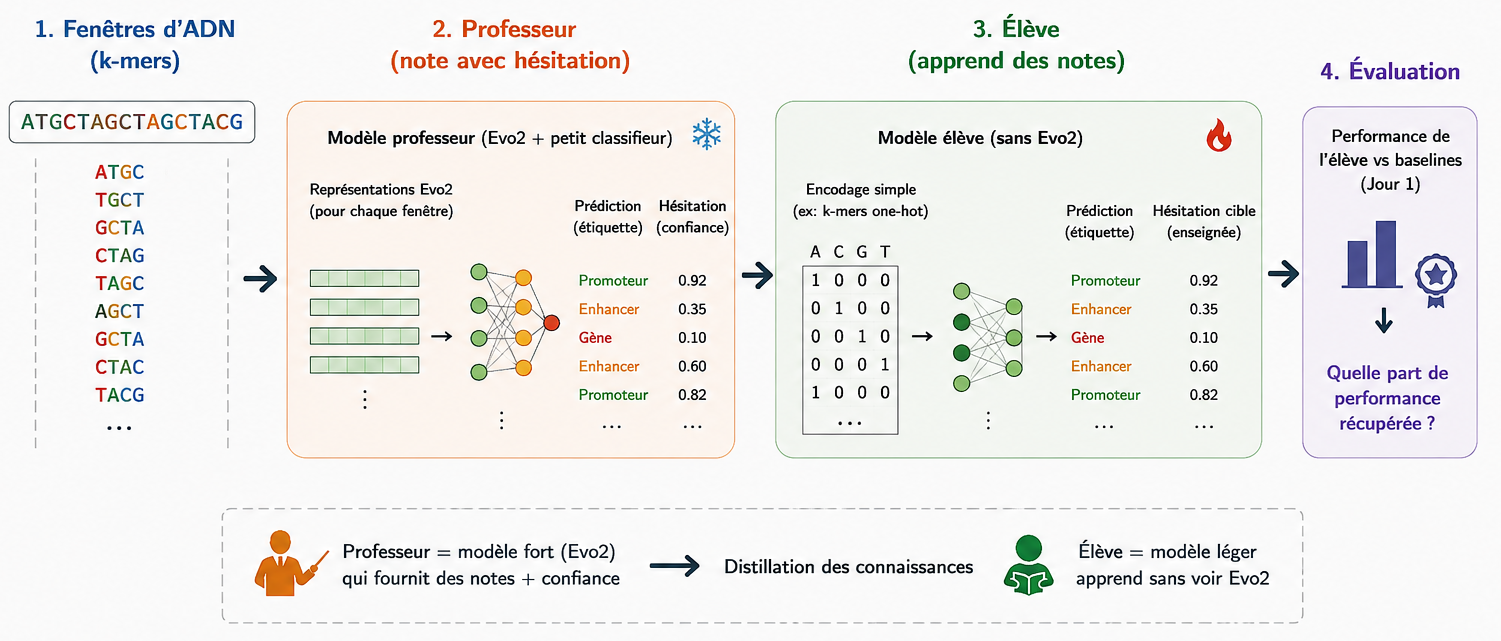
\includegraphics[height=5cm,keepaspectratio]{illustrations/lab3.png}}
    \only<4>{%
      \begin{itemize}
        \item Tous les modèles sur un seul graphique : précision, taille, latence
        \item \textbf{Que garderiez-vous} pour un appareil de terrain ?
      \end{itemize}}
    \only<5>{%
      \begin{itemize}
        \item Sans aucune étiquette, que le modèle a-t-il découvert tout seul ?
        \item Autoencodeurs parcimonieux sur les activations d'Evo2
      \end{itemize}
      \vspace{2pt}
      \centering
      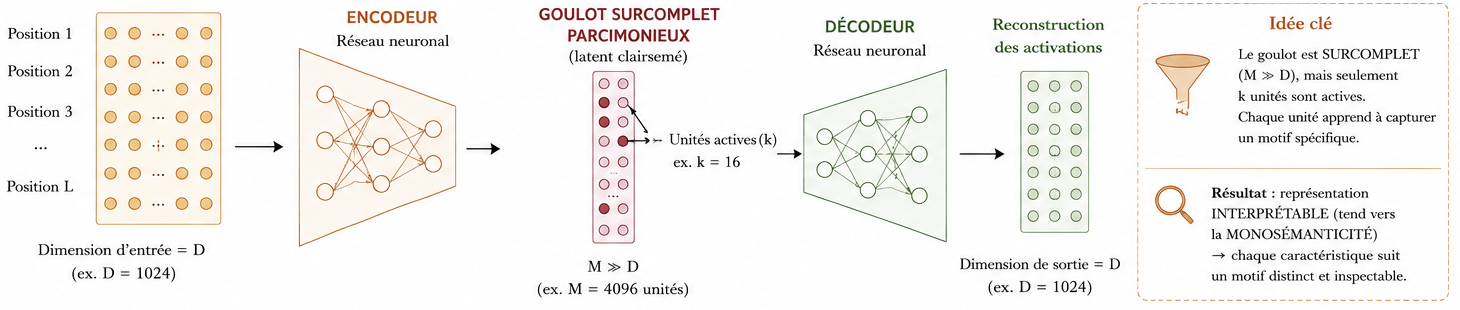
\includegraphics[width=10.5cm,keepaspectratio]{illustrations/sae.png}}
    \only<6>{%
      \begin{minipage}[t]{0.5\textwidth}
        \begin{itemize}
          \item Le même pipeline, appliqué aux \textbf{protéines}
          \item ESM2 (modèle de langage protéique) $\rightarrow$ embeddings
            $\rightarrow$ petit classifieur
          \item 8 familles de facteurs de transcription végétaux
          \item Une courte démo, \textbf{optionnelle}
        \end{itemize}
      \end{minipage}\hfill
      \begin{minipage}[t]{0.46\textwidth}
        \vspace{0pt}\centering
        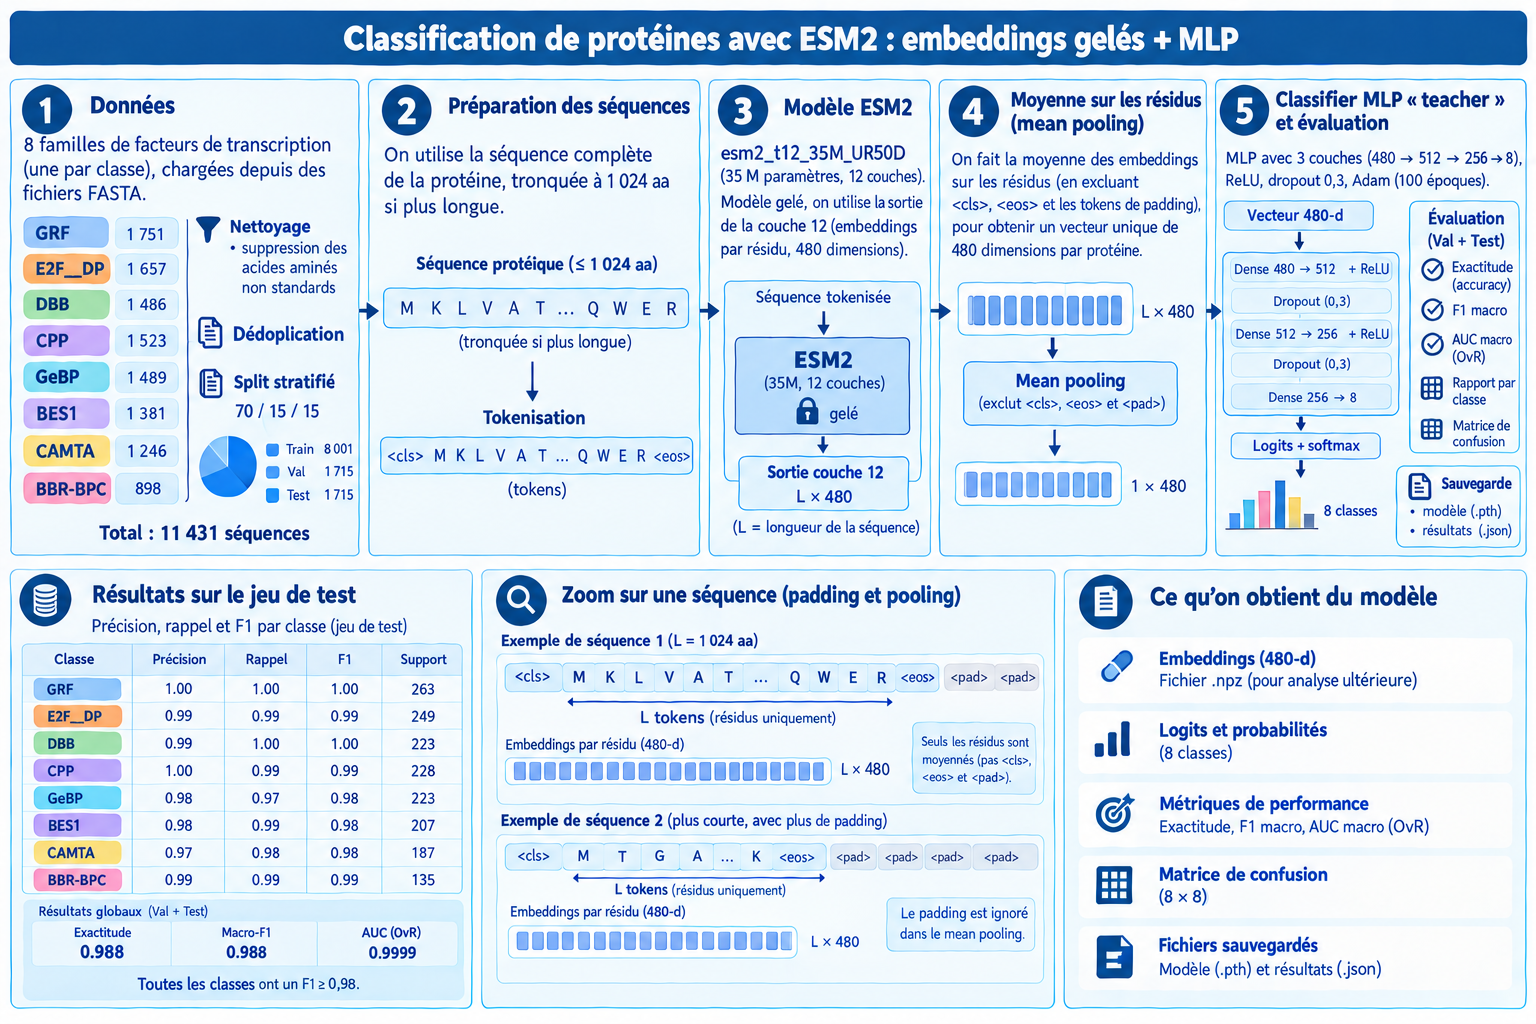
\includegraphics[height=3.8cm,keepaspectratio]{illustrations/lab-bonus-protein.png}
      \end{minipage}}
  \end{minipage}
\end{frame}

% =========================================================
{\setbeamercolor{background canvas}{bg=aliveblue}
 \setbeamertemplate{footline}{}
\begin{frame}[plain]
  \begin{tikzpicture}[remember picture,overlay]
    \node[anchor=east,opacity=0.30,inner sep=0pt]
      at ([xshift=1.7cm]current page.east)
      {
\includegraphics[height=1.06\paperheight]{illustrations/dna-light.png}};

    \node[anchor=west,text width=10.4cm,align=left]
      at ([shift={(1.05,-0.35)}]current page.west) {
      {\color{alivegold}\footnotesize\bfseries COMMENT ON TRAVAILLE\par}
      \vspace{0.35cm}
      {\color{white}\fontsize{26}{28}\selectfont\bfseries
       Vous complétez les trous, lab après lab.\par}
      \vspace{0.55cm}
      {\color{white!80}\fontsize{12.5}{16}\selectfont
       Chaque matin, un notebook \textbf{incomplet} vous attend : le squelette est
       là, les morceaux qui comptent sont à vous. Vous codez, nous
       passons si besoin, et le soir votre pipeline a avancé d'un cran.\par}
      \vspace{0.5cm}
      {\color{white!80}\fontsize{12.5}{16}\selectfont
       En trois jours, vous serez passés d'un génome brut à un modèle compressé
       que vous aurez construit, mesuré et compris.% --- et vous le présenterez.\par
       }
      % \vspace{0.85cm}
      % {\color{alivegold}\fontsize{15}{18}\selectfont\bfseries
      %  On vous attend.\par}
    };
  \end{tikzpicture}
\end{frame}}

\end{document}
